\documentclass[
]{jss}

%% recommended packages
\usepackage{orcidlink,thumbpdf,lmodern}

\usepackage[utf8]{inputenc}

\author{
Hanne I. Oberman\\Utrecht University \And Johanna Munoz Avila\\Julius
Center for Health Sciences and Primary Care,\\
University Medical Center Utrecht, Utrecht University,\\
Utrecht, The Netherlands \AND Thomas P. A. Debray\\Julius Center
for Health Sciences and Primary Care \And Gerko Vink\\Utrecht University
\AND Valentijn M. T. de Jong\\Julius Center for Health Sciences and
Primary Care,\\
University Medical Center Utrecht, Utrecht University,\\
Utrecht, The Netherlands
}
\title{Imputation of Incomplete Multilevel Data with \pkg{mice}}

\Plainauthor{Hanne I. Oberman, Johanna Munoz Avila, Thomas P. A.
Debray, Gerko Vink, Valentijn M. T. de Jong}
\Plaintitle{Imputation of Incomplete Multilevel Data with mice}
\Shorttitle{Multilevel \pkg{mice}}


\Abstract{
This tutorial illustrates the imputation of incomplete multilevel data
with the \proglang{R} packackage \pkg{mice}. Footnotes in the current
version show work in progress/under construction. The last section is
not part of the manuscript, but purely for reminders. See also all of
the TODOs that need to be worked out. We aim to submit at JSS, so there
is no word count limit (``There is no page limit, nor a limit on the
number of figures or tables''). {[}Just adding some text to get a better
guess of what the actura abstract will look like: Lorem ipsum dolor sit
amet, consectetur adipiscing elit, sed do eiusmod tempor incididunt ut
labore et dolore magna aliqua. Ut enim ad minim veniam, quis nostrud
exercitation ullamco laboris nisi ut aliquip ex ea commodo consequat.
Duis aute irure dolor in reprehenderit in voluptate velit esse cillum
dolore eu fugiat nulla pariatur. Excepteur sint occaecat cupidatat non
proident, sunt in culpa qui officia deserunt mollit anim id est
laborum.{]}
}

\Keywords{missing
data, multilevel, clustering, \pkg{mice}, \proglang{R}}
\Plainkeywords{missing data, multilevel, clustering, mice, R}

%% publication information
%% \Volume{50}
%% \Issue{9}
%% \Month{June}
%% \Year{2012}
%% \Submitdate{}
%% \Acceptdate{2012-06-04}

\Address{
    Hanne I. Oberman\\
    Utrecht University\\
    Padualaan 14\\
3584 CH Utrecht\\
  E-mail: \email{h.i.oberman@uu.nl}\\
  URL: \url{https://hanneoberman.github.io/}\\~\\
        Thomas P. A. Debray\\
    Julius Center for Health Sciences and Primary Care\\
    University Medical Center Utrecht, Utrecht University,\\
Utrecht, The Netherlands\\
  
  
      }


% tightlist command for lists without linebreak
\providecommand{\tightlist}{%
  \setlength{\itemsep}{0pt}\setlength{\parskip}{0pt}}



\usepackage{graphicx}
\usepackage{mathtools}
\usepackage{ulem}

\usepackage{amsmath}

\begin{document}



\hypertarget{introduction}{%
\section{Introduction}\label{introduction}}

Many datasets include individuals from multiple settings, geographic
regions, or even different studies. In the simplest case, individuals
(e.g., students) are nested within so-called clusters (e.g., school
classes). More complex clustered structures may occur when there are
multiple hierarchical levels (e.g., patients within hospitals within
regions or countries), or when the clustering is non-nested (e.g.,
electronic health record data from diverse settings and populations
within large databases). In general, individuals from the same cluster
tend to be more similar than individuals from other clusters. In
statistical terms, this implies that observations from the same cluster
are correlated. If this correlation is left unaddressed, estimates of
\emph{p} values, confidence intervals even model parameters are prone to
bias \citep{loca01}. {[}TODO: make a link to imputation methods, which
require adequate handling and propagation of variance; we are not
recommending the adoption of multilevel models for data analysis here,
but rather for imputation. VMTdJ: ``I would only make that link after
introducing missing data, and missing data is not mentioned yet, so I
would do that in the next section''{]} Statistical methods for clustered
data typically adopt hierarchical models that explicitly describe the
grouping of observations. These models are also known as `multilevel
models', `hierarchical models', `mixed effect models', `random effect
models', and in the context of time-to-event data as `frailty models'.
Table \ref{tab:clus} provides an overview of some key concepts in
multilevel modeling.

\begin{table}[tb]
\caption{Concepts in multilevel methods}
\label{tab:clus}
\centering
\begin{tabular}{ll}
\hline
\textbf{Concept} & \textbf{Details}   \\
\hline
ICC                 & The variability due to clustering is often measured by means of the \\
                    & intraclass coefficient (ICC). The ICC can be seen as the percentage \\
                    & of variance that can be attributed to the cluster-level, where a high \\
                    & ICC would indicate that a lot of variability is due to the cluster \\
                    & structure. \\
Random effect       & Multilevel models typically accommodate for variability by including \\
                    & a separate group mean for each cluster. In addition to random \\
                    & intercepts, multilevel models can also include random coefficients \\
                    & and heterogeneous residual error variances across clusters [see e.g. \\
                    & @gelm06, @hox17 and @jong21]. [TODO: add stratification.] \\
\hline
\end{tabular}
\end{table}

\hypertarget{missingness-in-multilevel-data}{%
\subsection{Missingness in multilevel
data}\label{missingness-in-multilevel-data}}

Like any other dataset, clustered datasets are prone to missing data.
Several strategies can be used to handle missing data, including
complete case analysis and imputation. We focus on the latter approach
and discuss statistical methods for replacing the missing data with one
or more plausible values. Afterwards, the completed data can be analyzed
as if they were completely observed. In contrast to single imputation
(where missing data are only replaced once), multiple imputation allows
to preserve uncertainty due to missingness and is therefore recommended
(c.f. Rubin 1976).

When clustered datasets are affected by missing values, we can
distinguish between two types of missing data: sporadic missingness and
systematic missingness \citep{resc13}. Sporadic missingness arises when
variables are missing for some but not all of the units in a cluster
\citep{buur18, jola18}. For example, it is possible that test results
are missing for several students in one or more classes. {[}TODO:
Provide an example for one of the case studies below.{]} When all
observations are missing within one or more clusters, data are
systematically missing. {[}TODO: Refer to Figure 1 and put
interpretation in the figure caption. VMTdJ: ``Mention in text that this
is sporadic missingness?''{]}

\begin{CodeChunk}
\begin{figure}

{\centering 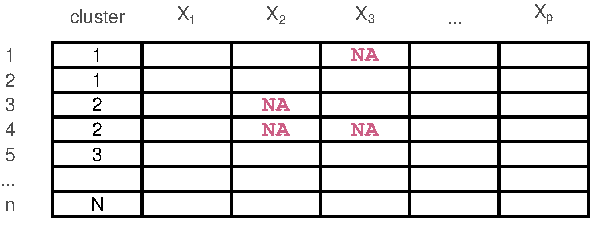
\includegraphics{Imputation_of_Incomplete_Multilevel_Data_files/figure-latex/patterns-1} 

}

\caption[Missingness in multilevel data]{Missingness in multilevel data}\label{fig:patterns}
\end{figure}
\end{CodeChunk}

Imputation of missing data requires consideration of the mechanism
behind the missingness. Rubin proposed to distinguish between data that
are missing completely at random (MCAR), data that are missing at random
(MAR) and data that are missing not at random (MNAR; see Table
\ref{tab:miss}). For each of these three missingness generating
mechanisms, different imputation strategies are warranted \citet{yuce08}
and \citet{hox15}. We here consider the general case that data are MAR,
and expand on certain MNAR situations.

\begin{table}[tb]
\caption{Concepts in missing data methods}
\label{tab:miss}
\centering
\begin{tabular}{ll}
\hline
\textbf{Concept} & \textbf{Details}   \\
\hline
MCAR    & Missing Completely At Random, where the probability to be missing is equal \\
& across all data entries \\
MAR     & Missing At Random, where the probability to be missing depends on observed \\
& information \\
MNAR    & Missing Not At Random (MNAR), where the probability to be missing \\
& depends on unrecorded information, making the missingness non-ignorable \\
& [@rubi76; @meng94]. \\
& [TODO: add congeniality, but maybe in-text?] \\
\hline
\end{tabular}
\end{table}

The \proglang{R} package \pkg{mice} has become the de-facto standard for
imputation by chained equations, which iteratively solves the
missingness on a variable-by-variable basis. \pkg{mice} is known to
yield valid inferences under many different missing data circumstances
\citep{buur18}. However, commonly used imputation methods were not
designed for use in clustered data and usually generate observations
that are independent whereas multilevel data are dependent. For this
reason, we discuss how the \proglang{R} package \pkg{mice} can be used
to impute multilevel data.

{[}TODO: clarify why clustering is relevant during imputation, and why
this exposes the need for specialized imputation methods and more
attention during their implementation (``thou shall not simply run
\texttt{mice()} on any incomplete dataset'').{]} {[}TODO: Add that the
more the random effects are of interest, the more you need multilevel
imputation models.{]} {[}TODO: Add an overview of all possible predictor
matrix values in manuscript or \texttt{ggmice} legend.{]}

\hypertarget{aim-of-this-paper}{%
\subsection{Aim of this paper}\label{aim-of-this-paper}}

This papers serves as a tutorial for imputing incomplete multilevel data
with \pkg{mice} in \proglang{R}. We provide practical guidelines and
code snippets for different missing data situations, including
non-ignorable mechanisms. For reasons of brevity, we focus on multilevel
imputation by chained equations with \pkg{mice} exclusively; other
imputation methods and packages (e.g., \pkg{jomo} and \pkg{mdmb}) are
outside the scope of this tutorial. {[}TODO: change this sentence
because we do not assume familiarity: ``Assumed knowledge includes basic
familiarity with multilevel imputation \citep[see e.g.][ and
\citet{grun18}]{audi18} and the \pkg{lme4} notation for multilevel
models (see Table \ref{tab:mod})''{]}.

\begin{table}[tb]
\caption{Notation}
\label{tab:mod}
\centering
\begin{tabular}{ll}
\hline
\textbf{Concept} & \textbf{Details}   \\
\hline
& [TODO: explain \pkg{lme4} notation here] \\
\hline
\end{tabular}
\end{table}

We illustrate imputation of incomplete multilevel data using three case
studies:

\begin{itemize}
\tightlist
\item
  \texttt{popmis} from the \pkg{mice} package \citep[simulated data on
  perceived popularity, \(n = 2,000\) pupils across \(N = 100\) schools
  with data that are MAR,][]{mice};
\item
  \texttt{impact} from the \pkg{metamisc} package \citep[empirical data
  on traumatic brain injuries, \(n = 11,022\) patients across \(N = 15\)
  studies with data that are MAR,][]{metamisc};
\item
  \texttt{hiv} from the \pkg{GJRM} package \citep[simulated data on HIV
  diagnoses, \(n = 6,416\) patients across \(N = 9\) regions with data
  that are MNAR,][]{GJRM}.
\end{itemize}

For each of these datasets, we discuss the nature of the missingness,
choose one or more imputation models and evaluate the imputed data, but
we will also highlight one specific aspect of the imputation workflow.

This tutorial is dedicated to readers who are unfamiliar with multiple
imputation. More experienced readers can skip the introduction (case
study 1) and directly head to practical applications of multilevel
imputation under MAR conditions (case study IMPACT) or under MNAR
conditions (case study HIV).

TODO: explicit statement about not going into workings of the methods.
Galimer 2l methods.

\hypertarget{setup}{%
\subsection{Setup}\label{setup}}

{[}TODO: Add environment info, seed and version number(s) somewhere.{]}
Set up the R environment and load the necessary packages:

\begin{CodeChunk}
\begin{CodeInput}
R> set.seed(2022)
R> library(mice)         # for imputation
R> library(miceadds)     # for imputation
R> library(ggmice)       # for visualization
R> library(ggplot2)      # for visualization
R> library(dplyr)        # for data wrangling
R> library(lme4)         # for multilevel modeling
R> library(mitml)        # for multilevel pooling
R> library(miceheckman)  # for imputation
\end{CodeInput}
\end{CodeChunk}

\hypertarget{case-study-i-popularity-data}{%
\section{Case study I: popularity
data}\label{case-study-i-popularity-data}}

{[}TODO: explain case study{]}

In this section we'll go over the different steps involved with imputing
incomplete multilevel data with the R package mice. We consider the
simulated \texttt{popmis} dataset, which included pupils (\(n = 2000\))
clustered within schools (\(N = 100\)). The following variables are of
primary interest:

\begin{itemize}
\tightlist
\item
  \texttt{school}, school identification number (clustering variable);
\item
  \texttt{popular}, pupil popularity (self-rating between 0 and 10;
  unit-level);
\item
  \texttt{sex}, pupil sex (0=boy, 1=girl; unit-level);
\item
  \texttt{texp}, teacher experience (in years; cluster-level).
\end{itemize}

The research objective of the \texttt{popmis} dataset is to predict the
pupils' popularity based on their gender and the experience of the
teacher. The analysis model corresponding to this dataset is multilevel
regression with random intercepts, random slopes and a cross-level
interaction. The outcome variable is \texttt{popular}, which is
predicted from the unit-level variable \texttt{sex} and the
cluster-level variable \texttt{texp}:

\begin{CodeChunk}
\begin{CodeInput}
R> mod <- popular ~ 1 + sex + (1 | school)
\end{CodeInput}
\end{CodeChunk}

The true effect is:

\begin{CodeChunk}


\begin{center}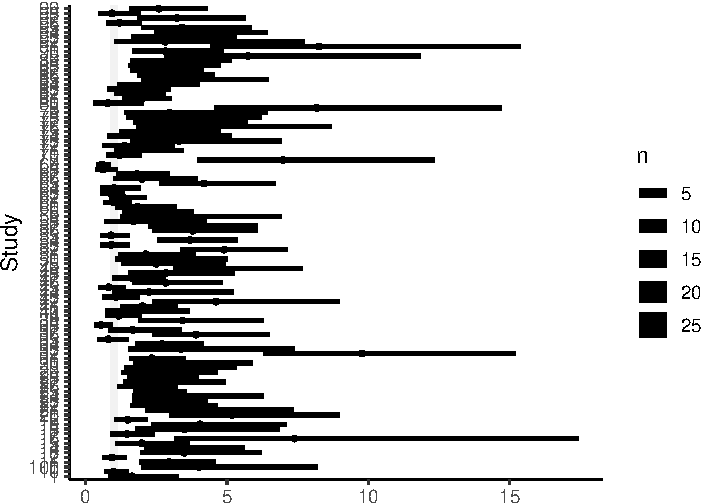
\includegraphics{Imputation_of_Incomplete_Multilevel_Data_files/figure-latex/unnamed-chunk-3-1} \end{center}

\end{CodeChunk}

Load the data into the environment and select the relevant variables:

\begin{CodeChunk}
\begin{CodeInput}
R> popmis <- popmis[, c("school", "popular", "sex")] 
\end{CodeInput}
\end{CodeChunk}

Plot the missing data pattern:

\begin{CodeChunk}
\begin{CodeInput}
R> plot_pattern(popmis)
\end{CodeInput}
\begin{figure}

{\centering 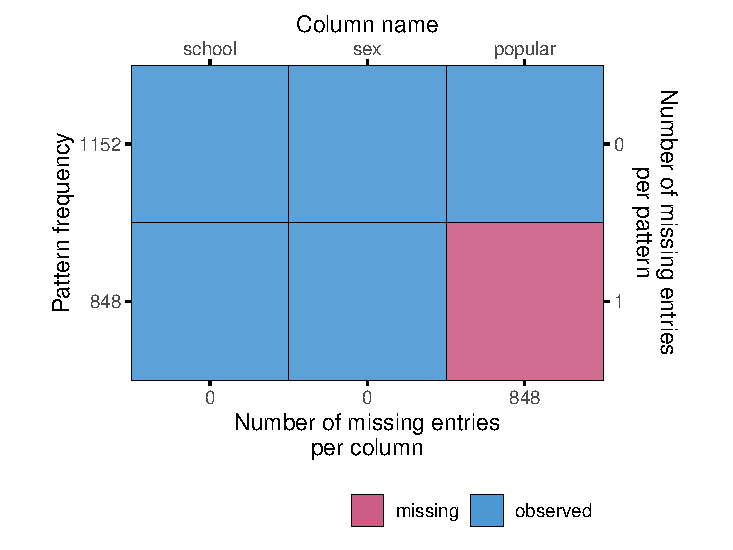
\includegraphics{Imputation_of_Incomplete_Multilevel_Data_files/figure-latex/pop_pat-1} 

}

\caption[Missing data pattern in the popularity data]{Missing data pattern in the popularity data}\label{fig:pop_pat}
\end{figure}
\end{CodeChunk}

The missingness is univariate and sporadic, which is illustrated in the
missing data pattern in Figure \ref{fig:pop_pat}.

To develop the best imputation model for the incomplete variable
\texttt{popular}, we need to know whether the observed values of
\texttt{popular} are related to observed values of other variables. Plot
the pair-wise complete correlations in the incomplete data:

\begin{CodeChunk}
\begin{CodeInput}
R> plot_corr(popmis)
\end{CodeInput}


\begin{center}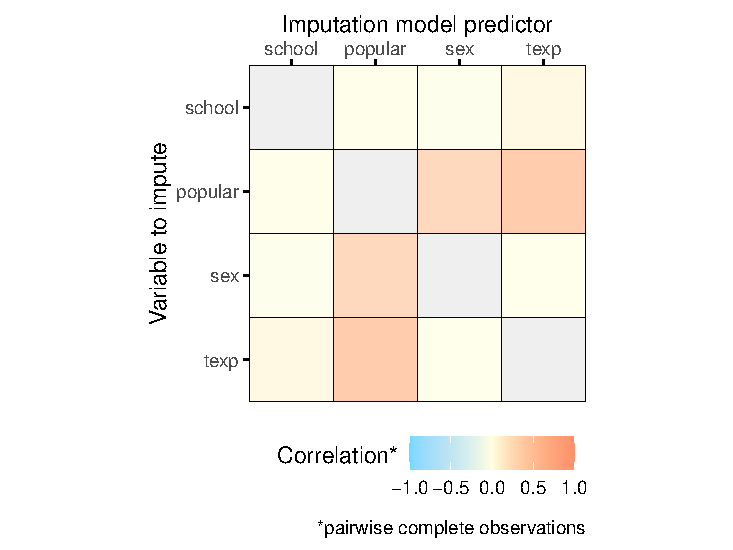
\includegraphics{Imputation_of_Incomplete_Multilevel_Data_files/figure-latex/pop-corr-1} \end{center}

\end{CodeChunk}

This shows us that \texttt{sex} may be a useful imputation model
predictor. Moreover, the missingness in \texttt{popular} may depend on
the observed values of other variables.

\begin{CodeChunk}
\begin{CodeInput}
R> # ggmice(popmis, aes(sex)) +
R> #   geom_histogram(fill = "white") +
R> #   facet_grid(. ~ is.na(popular), scales = "free", labeller = label_both)
R> 
R> ggplot(popmis, aes(y = popular, group = sex)) +
+   geom_boxplot() + 
+   theme_classic()
\end{CodeInput}


\begin{center}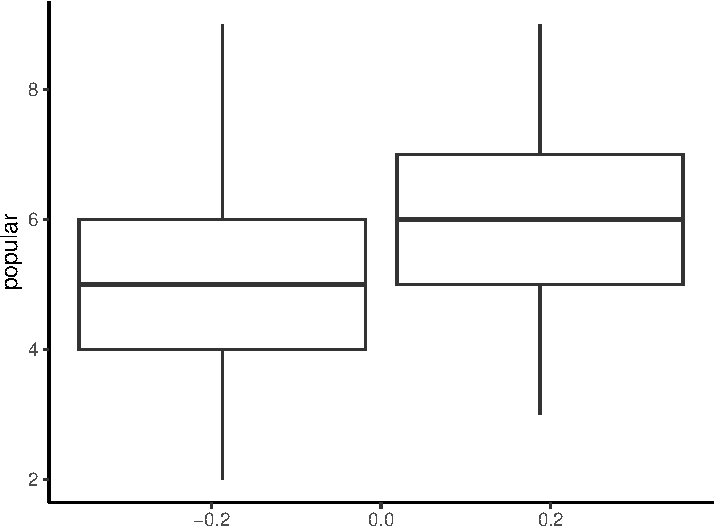
\includegraphics{Imputation_of_Incomplete_Multilevel_Data_files/figure-latex/pop-hist-1} \end{center}

\end{CodeChunk}

\hypertarget{imputation-ignoring-the-cluster-variable-not-recommended}{%
\subsubsection{Imputation ignoring the cluster variable (not
recommended)}\label{imputation-ignoring-the-cluster-variable-not-recommended}}

The first imputation model that we'll use is likely to be invalid. We do
\emph{not} use the cluster identifier \texttt{school} as imputation
model predictor. With this model, we ignore the multilevel structure of
the data, despite the high ICC. This assumes exchangeability between
units. We include it purely to illustrate the effects of ignoring the
clustering in our imputation effort.

Create a methods vector and predictor matrix for \texttt{popular}, and
make sure \texttt{school} is not included as predictor:

\begin{CodeChunk}
\begin{CodeInput}
R> meth <- make.method(popmis) # methods vector
R> pred <- quickpred(popmis)   # predictor matrix
R> plot_pred(pred)
\end{CodeInput}


\begin{center}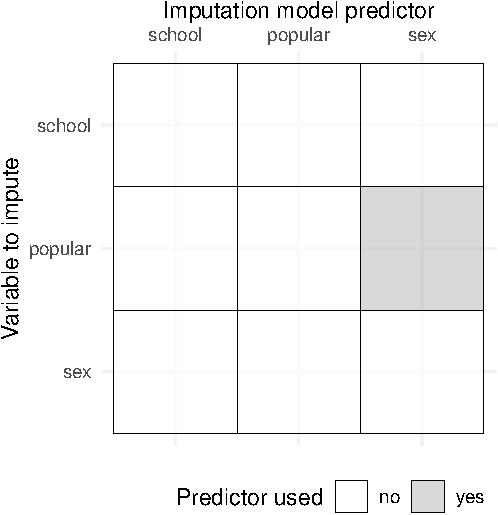
\includegraphics{Imputation_of_Incomplete_Multilevel_Data_files/figure-latex/pop-ignored-pred-1} \end{center}

\end{CodeChunk}

Impute the data, ignoring the cluster structure:

\begin{CodeChunk}
\begin{CodeInput}
R> imp <- mice(popmis, pred = pred, print = FALSE)
\end{CodeInput}
\end{CodeChunk}

Analyze the imputations:

\begin{CodeChunk}
\begin{CodeInput}
R> fit <- with(imp, 
+             lmer(popular ~ 1 + sex  + (1 | school))) 
\end{CodeInput}
\end{CodeChunk}

Print the estimates:

\begin{CodeChunk}
\begin{CodeInput}
R> testEstimates(as.mitml.result(fit), extra.pars = TRUE)
\end{CodeInput}
\begin{CodeOutput}

Call:

testEstimates(model = as.mitml.result(fit), extra.pars = TRUE)

Final parameter estimates and inferences obtained from 5 imputed data sets.

             Estimate Std.Error   t.value        df   P(>|t|)       RIV       FMI 
(Intercept)     5.012     0.295    16.994     4.362     0.000    22.587     0.969 
sex             0.695     0.251     2.768     4.287     0.047    28.390     0.975 

                            Estimate 
Intercept~~Intercept|school    0.266 
Residual~~Residual             1.035 
ICC|school                     0.208 

Unadjusted hypothesis test as appropriate in larger samples.
\end{CodeOutput}
\end{CodeChunk}

\hypertarget{imputation-with-the-cluster-variable-as-predictor-not-recommended}{%
\subsubsection{Imputation with the cluster variable as predictor (not
recommended)}\label{imputation-with-the-cluster-variable-as-predictor-not-recommended}}

We'll now use \texttt{school} as a predictor to impute all other
variables. This is still not recommended practice, since it only works
under certain circumstances and results may be biased
\citep{drec15, ende16}. But at least, it includes some multilevel
aspect. This method is also called `fixed cluster imputation', and uses
N-1 indicator variables representing allocation of N clusters as a fixed
factor in the model \citep{reit06, ende16}. Colloquially, this is
`multilevel imputation for dummies'.

{[}TODO: Add that it doesn't work with systematic missingness (only with
sporadic). There's some pros and cons, and it may not even differ much
if the number of clusters is low.{]}

\begin{CodeChunk}
\begin{CodeInput}
R> # adjust the predictor matrix
R> pred["popular", "school"] <- 1 
R> plot_pred(pred)
\end{CodeInput}


\begin{center}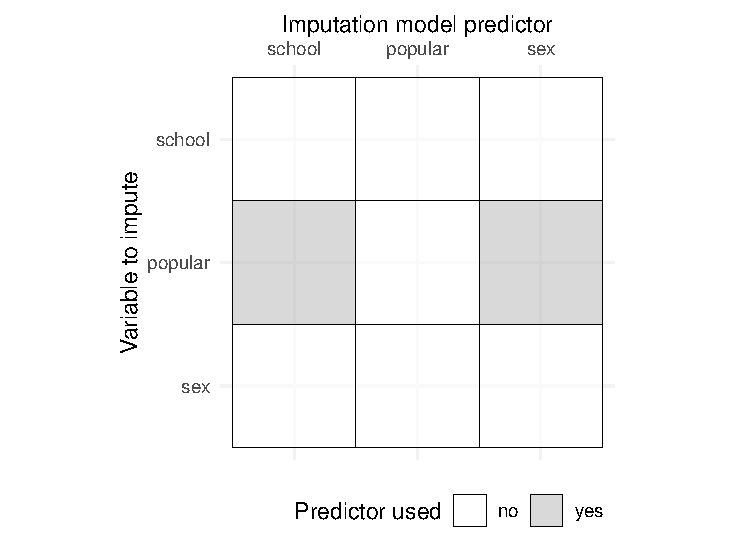
\includegraphics{Imputation_of_Incomplete_Multilevel_Data_files/figure-latex/pop_predictor-1} \end{center}

\begin{CodeInput}
R> # impute the data, cluster as predictor
R> imp <- mice(popmis, pred = pred, print = FALSE)
\end{CodeInput}
\end{CodeChunk}

Analyze the imputations:

\begin{CodeChunk}
\begin{CodeInput}
R> fit <- with(imp, 
+             lmer(popular ~ 1 + sex + (1 | school))) 
\end{CodeInput}
\end{CodeChunk}

Print the estimates:

\begin{CodeChunk}
\begin{CodeInput}
R> testEstimates(as.mitml.result(fit), extra.pars = TRUE)
\end{CodeInput}
\begin{CodeOutput}

Call:

testEstimates(model = as.mitml.result(fit), extra.pars = TRUE)

Final parameter estimates and inferences obtained from 5 imputed data sets.

             Estimate Std.Error   t.value        df   P(>|t|)       RIV       FMI 
(Intercept)     4.808     0.197    24.354     5.072     0.000     7.930     0.916 
sex             1.086     0.135     8.056     5.271     0.000     6.761     0.902 

                            Estimate 
Intercept~~Intercept|school    0.324 
Residual~~Residual             1.130 
ICC|school                     0.226 

Unadjusted hypothesis test as appropriate in larger samples.
\end{CodeOutput}
\end{CodeChunk}

\hypertarget{imputation-with-multilevel-model}{%
\subsubsection{Imputation with multilevel
model}\label{imputation-with-multilevel-model}}

\begin{CodeChunk}
\begin{CodeInput}
R> # adjust the predictor matrix
R> pred["popular", "school"] <- -2 
R> plot_pred(pred)
\end{CodeInput}


\begin{center}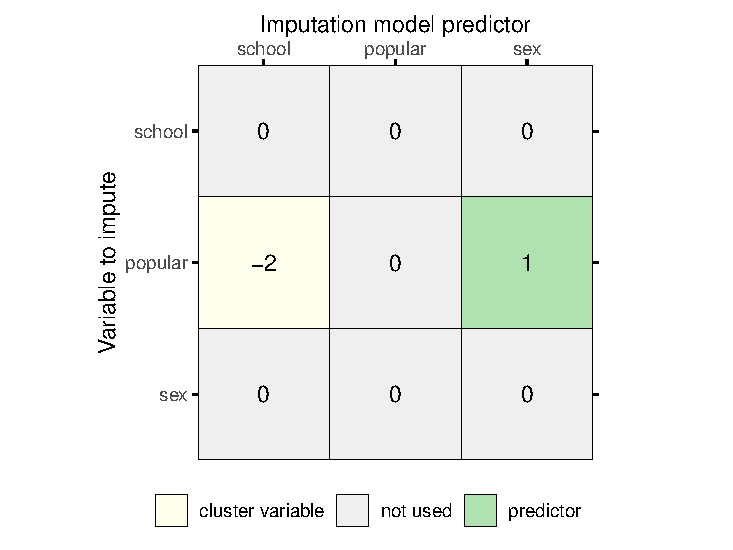
\includegraphics{Imputation_of_Incomplete_Multilevel_Data_files/figure-latex/pop_multilevel-1} \end{center}

\begin{CodeInput}
R> # impute the data, cluster as predictor
R> imp <- mice(popmis, pred = pred, print = FALSE)
\end{CodeInput}
\end{CodeChunk}

Analyze the imputations:

\begin{CodeChunk}
\begin{CodeInput}
R> fit <- with(imp, 
+             lmer(popular ~ 1 + sex + (1 | school))) 
\end{CodeInput}
\end{CodeChunk}

Print the estimates:

\begin{CodeChunk}
\begin{CodeInput}
R> testEstimates(as.mitml.result(fit), extra.pars = TRUE)
\end{CodeInput}
\begin{CodeOutput}

Call:

testEstimates(model = as.mitml.result(fit), extra.pars = TRUE)

Final parameter estimates and inferences obtained from 5 imputed data sets.

             Estimate Std.Error   t.value        df   P(>|t|)       RIV       FMI 
(Intercept)     4.808     0.197    24.354     5.072     0.000     7.930     0.916 
sex             1.086     0.135     8.056     5.271     0.000     6.761     0.902 

                            Estimate 
Intercept~~Intercept|school    0.324 
Residual~~Residual             1.130 
ICC|school                     0.226 

Unadjusted hypothesis test as appropriate in larger samples.
\end{CodeOutput}
\end{CodeChunk}

\hypertarget{case-study-ii-impact-data-syst-missingness-pred-matrix}{%
\section{Case study II: IMPACT data (syst missingness, pred
matrix)}\label{case-study-ii-impact-data-syst-missingness-pred-matrix}}

{[}TODO: check if there is systematic missingness in this dataset, if
not make Marshall Computerized Tomography classification (ct)
systematically missing.{]}

We illustrate how to impute incomplete multilevel data by means of a
case study: \texttt{impact} from the \pkg{metamisc} package
\citep[empirical data on traumatic brain injuries, \(n = 11,022\) units
across \(N = 15\) clusters,][]{metamisc}. {[}TODO: add more info about
the complete data.{]} The \texttt{impact} data set contains traumatic
brain injury data on \(n = 11022\) patients clustered in \(N = 15\)
studies with the following 11 variables:

\begin{itemize}
\tightlist
\item
  \texttt{name} Name of the study,
\item
  \texttt{type} Type of study (RCT: randomized controlled trial, OBS:
  observational cohort),
\item
  \texttt{age} Age of the patient,
\item
  \texttt{motor\_score} Glasgow Coma Scale motor score,
\item
  \texttt{pupil} Pupillary reactivity,
\item
  \texttt{ct} Marshall Computerized Tomography classification, {[}TODO:
  make this one var? also shows that you don't always need random
  effects everywhere?{]}
\item
  \texttt{hypox} Hypoxia (0=no, 1=yes),
\item
  \texttt{hypots} Hypotension (0=no, 1=yes),
\item
  \texttt{tsah} Traumatic subarachnoid hemorrhage (0=no, 1=yes),
\item
  \texttt{edh} Epidural hematoma (0=no, 1=yes),
\item
  \texttt{mort} 6-month mortality (0=alive, 1=dead).
\end{itemize}

The analysis model for this dataset is a prediction model with
\texttt{mort} as the outcome. In this tutorial we'll estimate the
adjusted prognostic effect of \texttt{ct} on mortality outcomes. The
estimand is the adjusted odds ratio for \texttt{ct}, after including
\texttt{type}, \texttt{age} \texttt{motor\_score} and \texttt{pupil}
into the analysis model:

\begin{CodeChunk}
\begin{CodeInput}
R> mod <- mort ~ 1 + type + age + motor_score + pupil + ct + (1 | name) 
\end{CodeInput}
\end{CodeChunk}

Note that variables \texttt{hypots}, \texttt{hypox}, \texttt{tsah} and
\texttt{edh} are not part of the analysis model, and may thus serve as
auxiliary variables for imputation.

The \texttt{impact} data included in the \pkg{metamisc} package is a
complete data set. The original data has already been imputed once
(Steyerberg et al, 2008). For the purpose of this tutorial we have
induced missingness (mimicking the missing data in the original data set
before imputation). The resulting incomplete data can be accessed from
\href{https://zenodo.com}{zenodo link to be created}.

Load the complete and incomplete data into the R workspace:

\begin{CodeChunk}
\begin{CodeInput}
R> data("impact", package = "metamisc")      # complete data
R> dat <- read.table("link/to/the/data.txt") # incomplete data
\end{CodeInput}
\end{CodeChunk}

The estimated effects in the complete data are visualized in Figure
\ref{}.

\begin{CodeChunk}


\begin{center}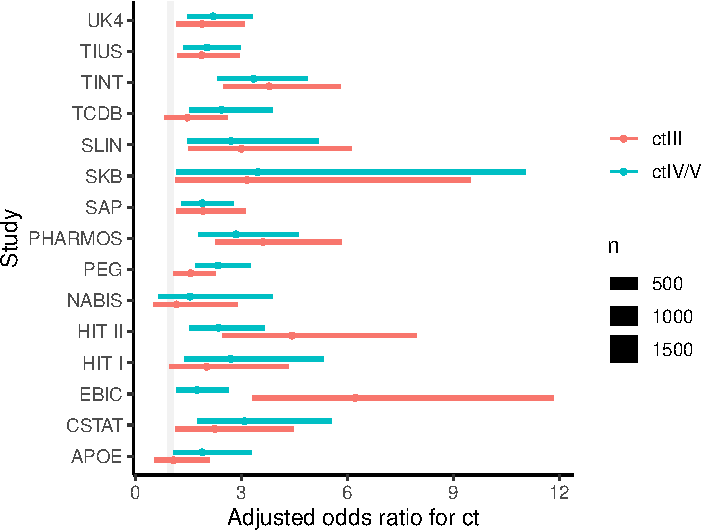
\includegraphics{Imputation_of_Incomplete_Multilevel_Data_files/figure-latex/forest-1} \end{center}

\end{CodeChunk}

\begin{CodeChunk}
\begin{CodeInput}
R> # fit <- glmer(mod, family = "binomial", data = impact) # fit the model
R> # tidy(fit, conf.int = TRUE, exponentiate = TRUE)       # print estimates
\end{CodeInput}
\end{CodeChunk}

{[}TODO: show how much variance there is after different methods{]}

{[}TODO: add ICC before/after imputation and interpret: This tells us
that the multilevel structure of the data should probably be taken into
account. If we don't, we'll may end up with incorrect imputations,
biasing the effect of the clusters towards zero.{]}

{[}TODO: add descriptive statistics of the complete and incomplete
data.{]}

\hypertarget{missingness}{%
\subsection{Missingness}\label{missingness}}

To explore the missingness, it is wise to look at the missing data
pattern:

\begin{CodeChunk}
\begin{CodeInput}
R> plot_pattern(dat, rotate = TRUE, npat = 10L)  # plot missingness pattern
\end{CodeInput}


\begin{center}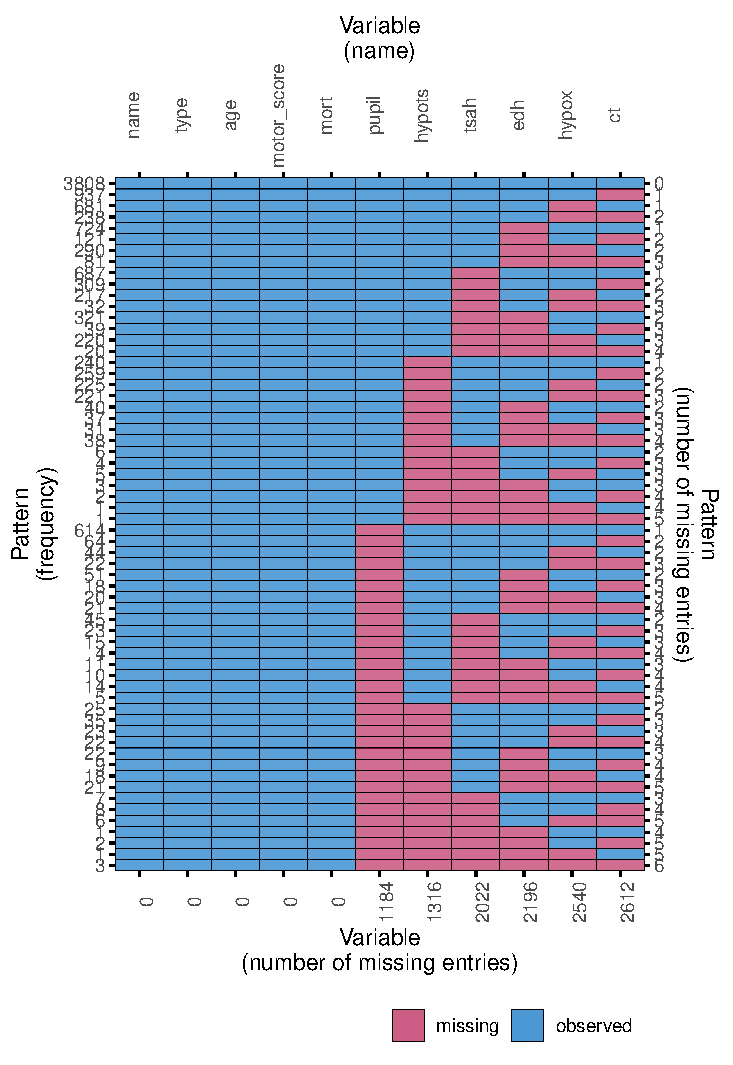
\includegraphics{Imputation_of_Incomplete_Multilevel_Data_files/figure-latex/pattern-1} \end{center}

\end{CodeChunk}

This shows\ldots{} {[}TODO: fill in that we need to impute \texttt{ct}
and \texttt{pupil}.{]}

To develop the best imputation model, we need to investigate the
relations between the observed values of the incomplete variables and
the observed values of other variables, and the relation between the
missingness indicators of the incomplete variables and the observed
values of the other variables. To see whether the missingness depends on
the observed values of other variables, we\ldots{} {[}TODO: fill in that
we can test this statistically or use visual inspection (e.g.~a
histogram faceted by the missingness indicator).{]}

We should impute the variables \texttt{ct} and \texttt{pupil} and any
auxiliary variables we might want to use to impute these incomplete
analysis model variables. We can evaluate which variables may be useful
auxiliaries by plotting the pairwise complete correlations:

\begin{CodeChunk}
\begin{CodeInput}
R> plot_corr(dat, rotate = TRUE) # plot correlations 
\end{CodeInput}


\begin{center}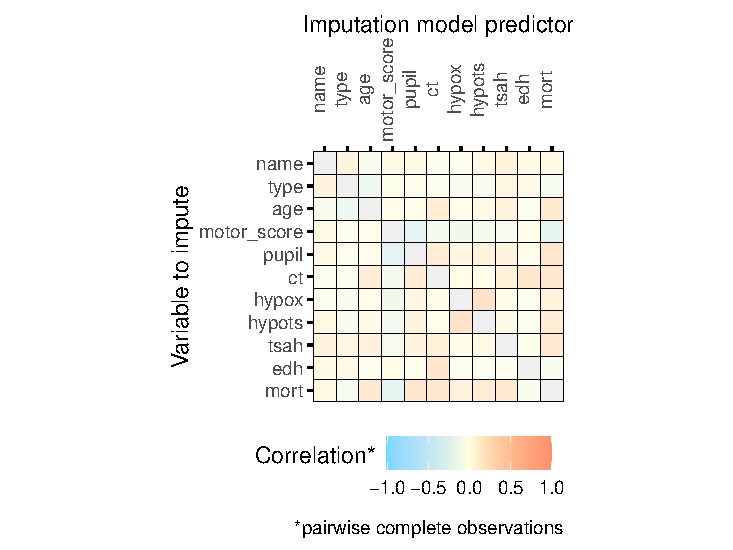
\includegraphics{Imputation_of_Incomplete_Multilevel_Data_files/figure-latex/impact_corr-1} \end{center}

\end{CodeChunk}

This shows us that \texttt{hypox} and \texttt{hypot} would not be useful
auxiliary variables for imputing \texttt{ct}. Depending on the minimum
required correlation, \texttt{tsah} could be useful, while \texttt{edh}
has the strongest correlation with \texttt{ct} out of all the variables
in the data and should definitely be included in the imputation model.
For the imputation of \texttt{pupil}, none of the potential auxiliary
variables has a very strong relation, but \texttt{hypots} could be used.
We conclude that we can exclude \texttt{hypox} from the data, since this
is neither an analysis model variable nor an auxiliary variable for
imputation:

\begin{CodeChunk}
\begin{CodeInput}
R> dat <- select(dat, !hypox)  # remove variable
\end{CodeInput}
\end{CodeChunk}

\hypertarget{complete-case-analysis-todo-remove-this}{%
\subsection{Complete case analysis {[}TODO: remove
this?{]}}\label{complete-case-analysis-todo-remove-this}}

As previously stated, complete case analysis lowers statistical power
and may bias results. The complete case analysis estimates are:

\begin{CodeChunk}
\begin{CodeInput}
R> fit <- glmer(mod, family = "binomial", data = na.omit(dat)) # fit the model
R> tidy(fit, conf.int = TRUE, exponentiate = TRUE)             # print estimates
\end{CodeInput}
\begin{CodeOutput}
# A tibble: 11 x 9
   effect   group term        estim~1 std.er~2 stati~3   p.value conf.~4 conf.~5
   <chr>    <chr> <chr>         <dbl>    <dbl>   <dbl>     <dbl>   <dbl>   <dbl>
 1 fixed    <NA>  (Intercept)  0.0863  0.0182   -11.6   2.99e-31  0.0571   0.130
 2 fixed    <NA>  typeRCT      0.757   0.137     -1.54  1.22e- 1  0.531    1.08 
 3 fixed    <NA>  age          1.03    0.00265   12.9   7.40e-38  1.03     1.04 
 4 fixed    <NA>  motor_scor~  0.651   0.0732    -3.82  1.34e- 4  0.522    0.811
 5 fixed    <NA>  motor_scor~  0.489   0.0555    -6.30  2.97e-10  0.391    0.611
 6 fixed    <NA>  motor_scor~  0.274   0.0321   -11.0   2.28e-28  0.218    0.345
 7 fixed    <NA>  pupilNone    3.20    0.317     11.7   8.18e-32  2.63     3.88 
 8 fixed    <NA>  pupilOne     1.75    0.195      5.06  4.27e- 7  1.41     2.18 
 9 fixed    <NA>  ctIII        2.41    0.268      7.89  3.05e-15  1.94     2.99 
10 fixed    <NA>  ctIV/V       2.30    0.214      8.95  3.55e-19  1.92     2.76 
11 ran_pars name  sd__(Inter~  0.230  NA         NA    NA        NA       NA    
# ... with abbreviated variable names 1: estimate, 2: std.error, 3: statistic,
#   4: conf.low, 5: conf.high
\end{CodeOutput}
\end{CodeChunk}

As we can see\ldots{} {[}TODO: fill in: This means that a higher ct
(Marshall Computerized Tomography classification) is associated with a
lower odds of 6-month mortality, given by the odds ratio exp(0.42), CI
\ldots{} to \ldots, when controlling for \ldots{]}

\hypertarget{imputation-model}{%
\subsection{Imputation model}\label{imputation-model}}

Mutate data to get the right data types for imputation (e.g.~integer for
clustering variable).

\begin{CodeChunk}
\begin{CodeInput}
R> dat <- dat %>% mutate(across(everything(), as.integer))
\end{CodeInput}
\end{CodeChunk}

Create a methods vector and predictor matrix, and make sure
\texttt{name} is not included as predictor, but as clustering variable:

\begin{CodeChunk}
\begin{CodeInput}
R> meth <- make.method(dat) # methods vector
R> pred <- quickpred(dat)   # predictor matrix
R> plot_pred(pred)
\end{CodeInput}


\begin{center}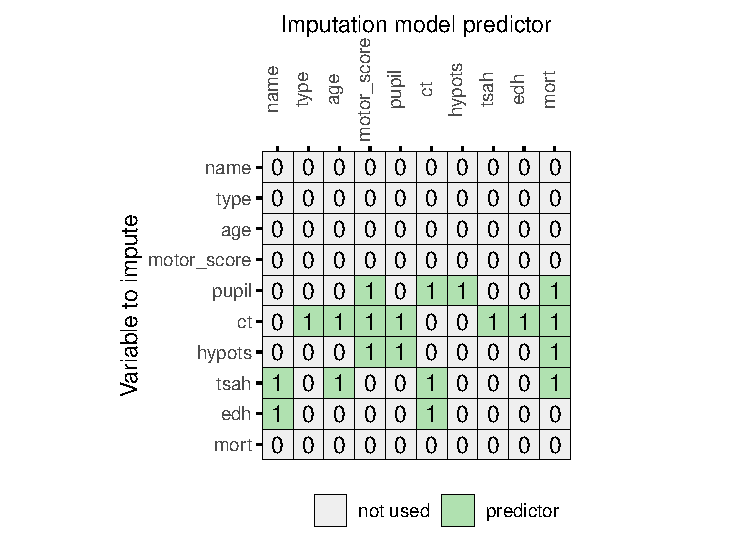
\includegraphics{Imputation_of_Incomplete_Multilevel_Data_files/figure-latex/impact-1} \end{center}

\begin{CodeInput}
R> pred[pred == 1] <- 2
R> pred["mort", ] <- 2
R> pred[, "mort"] <- 2
R> pred[c("name", "type", "age", "motor_score", "mort"), ] <- 0
R> pred[, "name"] <- -2
R> diag(pred) <- 0
R> plot_pred(pred)
\end{CodeInput}


\begin{center}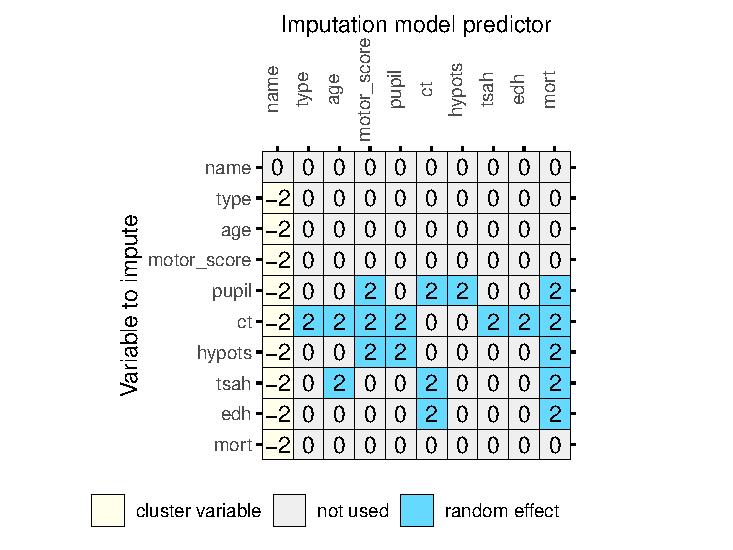
\includegraphics{Imputation_of_Incomplete_Multilevel_Data_files/figure-latex/impact-2} \end{center}

\begin{CodeInput}
R> meth <- make.method(dat)
R> meth
\end{CodeInput}
\begin{CodeOutput}
       name        type         age motor_score       pupil          ct 
         ""          ""          ""          ""       "pmm"       "pmm" 
     hypots        tsah         edh        mort 
      "pmm"       "pmm"       "pmm"          "" 
\end{CodeOutput}
\end{CodeChunk}

Impute the incomplete data

\begin{CodeChunk}
\begin{CodeInput}
R> imp <- mice(dat, method = meth, predictorMatrix = pred, printFlag = FALSE)
\end{CodeInput}
\end{CodeChunk}

\begin{CodeChunk}
\begin{CodeInput}
R> fit <- imp %>% 
+   with(glmer(mort ~ type + age + as.factor(motor_score) + pupil + ct + (1 | name), family = "binomial")) 
R> tidy(pool(fit))
\end{CodeInput}
\begin{CodeOutput}
                     term   estimate   std.error  statistic      p.value
1             (Intercept) -2.3054756 0.340854445  -6.763813 1.425704e-11
2                    type -0.4200458 0.180837517  -2.322780 2.021049e-02
3                     age  0.0302518 0.001561625  19.372002 0.000000e+00
4 as.factor(motor_score)2 -0.6619736 0.069527977  -9.520967 0.000000e+00
5 as.factor(motor_score)3 -1.0520025 0.070748986 -14.869507 0.000000e+00
6 as.factor(motor_score)4 -1.5087772 0.072240455 -20.885489 0.000000e+00
7                   pupil  0.4731045 0.038187004  12.389150 0.000000e+00
8                      ct  0.4291135 0.032126389  13.357041 0.000000e+00
             b          df dfcom         fmi      lambda m         riv
1 7.937082e-04  9227.60708 11013 0.008412824 0.008197930 5 0.008265691
2 1.386594e-04 10229.67142 11013 0.005282534 0.005088076 5 0.005114097
3 1.138007e-08 10083.78177 11013 0.005796971 0.005599802 5 0.005631337
4 1.427540e-04  2450.43742 11013 0.036222753 0.035436457 5 0.036738334
5 1.147119e-04  3540.28145 11013 0.028049975 0.027501049 5 0.028278744
6 1.377409e-04  2902.11217 11013 0.032339200 0.031672563 5 0.032708526
7 3.160434e-04    58.71181 11013 0.284053948 0.260073900 5 0.351486317
8 1.985834e-04    74.37520 11013 0.250767587 0.230887509 5 0.300199921
          ubar
1 1.152293e-01
2 3.253582e-02
3 2.425016e-06
4 4.662835e-03
5 4.867765e-03
6 5.053394e-03
7 1.078995e-03
8 7.938047e-04
\end{CodeOutput}
\begin{CodeInput}
R> as.mitml.result(fit)
\end{CodeInput}
\begin{CodeOutput}
[[1]]
Generalized linear mixed model fit by maximum likelihood (Laplace
  Approximation) [glmerMod]
 Family: binomial  ( logit )
Formula: mort ~ type + age + as.factor(motor_score) + pupil + ct + (1 |  
    name)
      AIC       BIC    logLik  deviance  df.resid 
10494.825 10560.593 -5238.412 10476.825     11013 
Random effects:
 Groups Name        Std.Dev.
 name   (Intercept) 0.2917  
Number of obs: 11022, groups:  name, 15
Fixed Effects:
            (Intercept)                     type                      age  
               -2.33693                 -0.43143                  0.03013  
as.factor(motor_score)2  as.factor(motor_score)3  as.factor(motor_score)4  
               -0.67764                 -1.05120                 -1.49989  
                  pupil                       ct  
                0.49336                  0.44123  
optimizer (Nelder_Mead) convergence code: 0 (OK) ; 0 optimizer warnings; 2 lme4 warnings 

[[2]]
Generalized linear mixed model fit by maximum likelihood (Laplace
  Approximation) [glmerMod]
 Family: binomial  ( logit )
Formula: mort ~ type + age + as.factor(motor_score) + pupil + ct + (1 |  
    name)
      AIC       BIC    logLik  deviance  df.resid 
10543.607 10609.376 -5262.803 10525.607     11013 
Random effects:
 Groups Name        Std.Dev.
 name   (Intercept) 0.2937  
Number of obs: 11022, groups:  name, 15
Fixed Effects:
            (Intercept)                     type                      age  
               -2.28159                 -0.42088                  0.03026  
as.factor(motor_score)2  as.factor(motor_score)3  as.factor(motor_score)4  
               -0.65610                 -1.04928                 -1.49432  
                  pupil                       ct  
                0.48055                  0.41014  
optimizer (Nelder_Mead) convergence code: 0 (OK) ; 0 optimizer warnings; 1 lme4 warnings 

[[3]]
Generalized linear mixed model fit by maximum likelihood (Laplace
  Approximation) [glmerMod]
 Family: binomial  ( logit )
Formula: mort ~ type + age + as.factor(motor_score) + pupil + ct + (1 |  
    name)
      AIC       BIC    logLik  deviance  df.resid 
10543.170 10608.939 -5262.585 10525.170     11013 
Random effects:
 Groups Name        Std.Dev.
 name   (Intercept) 0.2901  
Number of obs: 11022, groups:  name, 15
Fixed Effects:
            (Intercept)                     type                      age  
               -2.29948                 -0.40181                  0.03038  
as.factor(motor_score)2  as.factor(motor_score)3  as.factor(motor_score)4  
               -0.65959                 -1.06391                 -1.52075  
                  pupil                       ct  
                0.45837                  0.42186  
optimizer (Nelder_Mead) convergence code: 0 (OK) ; 0 optimizer warnings; 2 lme4 warnings 

[[4]]
Generalized linear mixed model fit by maximum likelihood (Laplace
  Approximation) [glmerMod]
 Family: binomial  ( logit )
Formula: mort ~ type + age + as.factor(motor_score) + pupil + ct + (1 |  
    name)
      AIC       BIC    logLik  deviance  df.resid 
10527.222 10592.991 -5254.611 10509.222     11013 
Random effects:
 Groups Name        Std.Dev.
 name   (Intercept) 0.2962  
Number of obs: 11022, groups:  name, 15
Fixed Effects:
            (Intercept)                     type                      age  
               -2.27660                 -0.42912                  0.03016  
as.factor(motor_score)2  as.factor(motor_score)3  as.factor(motor_score)4  
               -0.66963                 -1.05952                 -1.51971  
                  pupil                       ct  
                0.45085                  0.44439  
optimizer (Nelder_Mead) convergence code: 0 (OK) ; 0 optimizer warnings; 1 lme4 warnings 

[[5]]
Generalized linear mixed model fit by maximum likelihood (Laplace
  Approximation) [glmerMod]
 Family: binomial  ( logit )
Formula: mort ~ type + age + as.factor(motor_score) + pupil + ct + (1 |  
    name)
      AIC       BIC    logLik  deviance  df.resid 
10519.178 10584.947 -5250.589 10501.178     11013 
Random effects:
 Groups Name        Std.Dev.
 name   (Intercept) 0.2897  
Number of obs: 11022, groups:  name, 15
Fixed Effects:
            (Intercept)                     type                      age  
               -2.33278                 -0.41699                  0.03032  
as.factor(motor_score)2  as.factor(motor_score)3  as.factor(motor_score)4  
               -0.64691                 -1.03611                 -1.50921  
                  pupil                       ct  
                0.48240                  0.42794  
optimizer (Nelder_Mead) convergence code: 0 (OK) ; 0 optimizer warnings; 1 lme4 warnings 

attr(,"class")
[1] "mitml.result" "list"        
\end{CodeOutput}
\begin{CodeInput}
R> # testEstimates(as.mitml.result(fit))
\end{CodeInput}
\end{CodeChunk}

\hypertarget{case-study-iii-hiv-data}{%
\section{Case study III: HIV data}\label{case-study-iii-hiv-data}}

Data are simulated and included in the \texttt{GJRM} package. We will
use the following variables:

\begin{itemize}
\tightlist
\item
  \texttt{region} Cluster variable,
\item
  \texttt{hiv} HIV diagnosis (0=no, 1=yes),
\item
  \texttt{age} Age of the patient,
\item
  \texttt{marital} Marital status,
\item
  \texttt{condom} Condom use during last intercourse,
\item
  \texttt{smoke} Smoker (levels; inclusion restriction variable).
\end{itemize}

The imputation of these date is based on the toy example from
\href{https://github.com/johamunoz/Heckman-IPDMA/blob/main/Toy_example.R}{IPDMA
Heckman Github repo}.

\begin{CodeChunk}


\begin{center}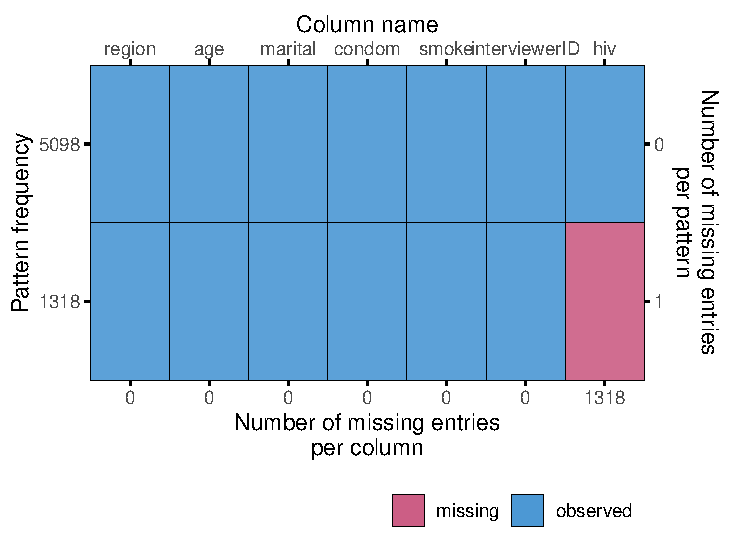
\includegraphics{Imputation_of_Incomplete_Multilevel_Data_files/figure-latex/hiv-1} \end{center}

\end{CodeChunk}

R=region+language+(1\textbar InterviewID) model with interviewer as
random effects, because the observations are not independent. Interviews
are not allocated randomly. In theory we expect the
inclusion-restriction variable to be randomly assigned, that's why we're
adding region and language to compensate for non-random allocation.
{[}TODO: Explain exclusion-restriction, refer to paper Johanna{]}.

Load the data:

\begin{CodeChunk}
\begin{CodeInput}
R> data("obesity",  package = "miceheckman")
\end{CodeInput}
\end{CodeChunk}

We obtain here the random effects for each interviewer, this is an
approximation of the interviewer's skill which will be used as an
exclusion constraint. Here, since the location of the interviewer was
not randomly assigned to the subjects, the assignment was corrected for
region and language.

Set the Heckman model as imputation method

\begin{CodeChunk}
\begin{CodeInput}
R> #Set prediction matrix and methods
R> ini <- mice(obesity, maxit = 0)
R> meth<-ini$method
R> meth["weight"]<-"2l.heckman"
R> pred <- ini$pred
R> pred["weight","cluster"]<- -2
R> pred["weight","rt"] <- -3
\end{CodeInput}
\end{CodeChunk}

Impute the data:

\begin{CodeChunk}
\begin{CodeInput}
R> imp <- mice(obesity, # dataset with missing values
+                         m = 10,   # number of imputations
+                         maxit = 1,
+                         seed = 1234, #seed attached to the dataID
+                         meth = meth, #imputation method vector
+                         pred = pred, #imputation predictors matrix
+                         print = T,
+                         meta_method="reml",
+                         pmm=FALSE)
\end{CodeInput}
\end{CodeChunk}

\hypertarget{discussion}{%
\section{Discussion}\label{discussion}}

\begin{itemize}
\item
  JOMO in \pkg{mice} -\textgreater{} on the side for now
\item
  Additional levels of clustering
\item
  More complex data types: timeseries and polynomial relationship in the
  clustering.
\end{itemize}

\hypertarget{think-about}{%
\section{Think about}\label{think-about}}

\begin{itemize}
\item
  Adding evaluations of the imputations such as convergence checks
\item
  Adding some kind of help function to mice that suggests a suitable
  predictor matrix to the user, given a certain analysis model.
\item
  Adding a \texttt{multilevel\_ampute()} wrapper function in mice.
\item
  Exporting \texttt{mids} objects to other packages like \texttt{lme4}
  or \texttt{coxme}?
\item
  Adding a ICC=0 dataset to show that even if there is no clustering it
  doesn't hurt.
\item
  Show use case for deductive imputation for cluster level variables?
\item
  env dump in repo
\end{itemize}

\hypertarget{funding}{%
\section{Funding}\label{funding}}

This project has received funding from the European Union's Horizon 2020
research and innovation programme under ReCoDID grant agreement No
825746.

The views expressed in this paper are the personal views of the authors
and may not be understood or quoted as being made on behalf of or
reflecting the position of the regulatory agency/agencies or
organizations with which the authors are employed/affiliated.

\renewcommand\refname{References}
\bibliography{../References/multilevelmice.bib}



\end{document}
